
\chapter{Introduction}
\section{Motivation}

The upcoming High Luminosity phase of the Large Hadron Collider (LHC)~\cite{LHC_machine_2008} presents unprecedented opportunities to explore new physics in ATLAS~\cite{collaboration_atlas_2008} and CMS~\cite{CMS_2008}. The increased luminosity enables the collection of vast experimental data, with Run 3 nearly doubling the luminosity of Run 2~\cite{Future_LHC}.

At higher collision rates, the LHC will generate approximately 1 billion proton-proton (p-p) collisions per second, captured by detectors with nearly 100 million readout channels. With just 25 nanoseconds between successive proton bunches, new collisions occur before previous interactions fully exit the detector. This immense data volume provides rich opportunities for discovery but also introduces significant challenges in data processing, storage, and simulation.

\subsection{The Role of Simulation in High-Energy Physics}

Simulation plays a critical role in high-energy physics, allowing researchers to compare experimental data with theoretical predictions. Every study must first validate that observed data aligns with background expectations and signals, ensuring a clear understanding of each channel’s contributions. However, traditional simulation methods face computational bottlenecks, particularly as data rates increase. Accelerating simulation without sacrificing accuracy is essential for timely and reliable analysis.

Monte Carlo-based methods, such as those implemented in Geant4~\cite{Geant4}, have long been the standard for simulating particle interactions and detector responses. These simulations provide high precision but are computationally expensive and struggle to keep pace with increasing data rates. As detector complexity grows, the time required for full simulations rises, making it increasingly difficult to scale traditional techniques to modern experimental demands.

A significant portion of high-energy physics computing resources is devoted to simulating particle propagation in dense materials, particularly within calorimeters, which measure deposited energy. Simulating electromagnetic and nuclear interactions in these dense environments is particularly challenging, requiring extensive computational power. Given the constraints on computing budgets, full Geant4 simulations are impractical for all events, leading to the development of fast simulation techniques. These methods replace detailed physics-based models with simplified parameterized approaches, which, while efficient, often fail to capture high-dimensional correlations and complex particle interactions.

\begin{figure}[H]
    \centering
    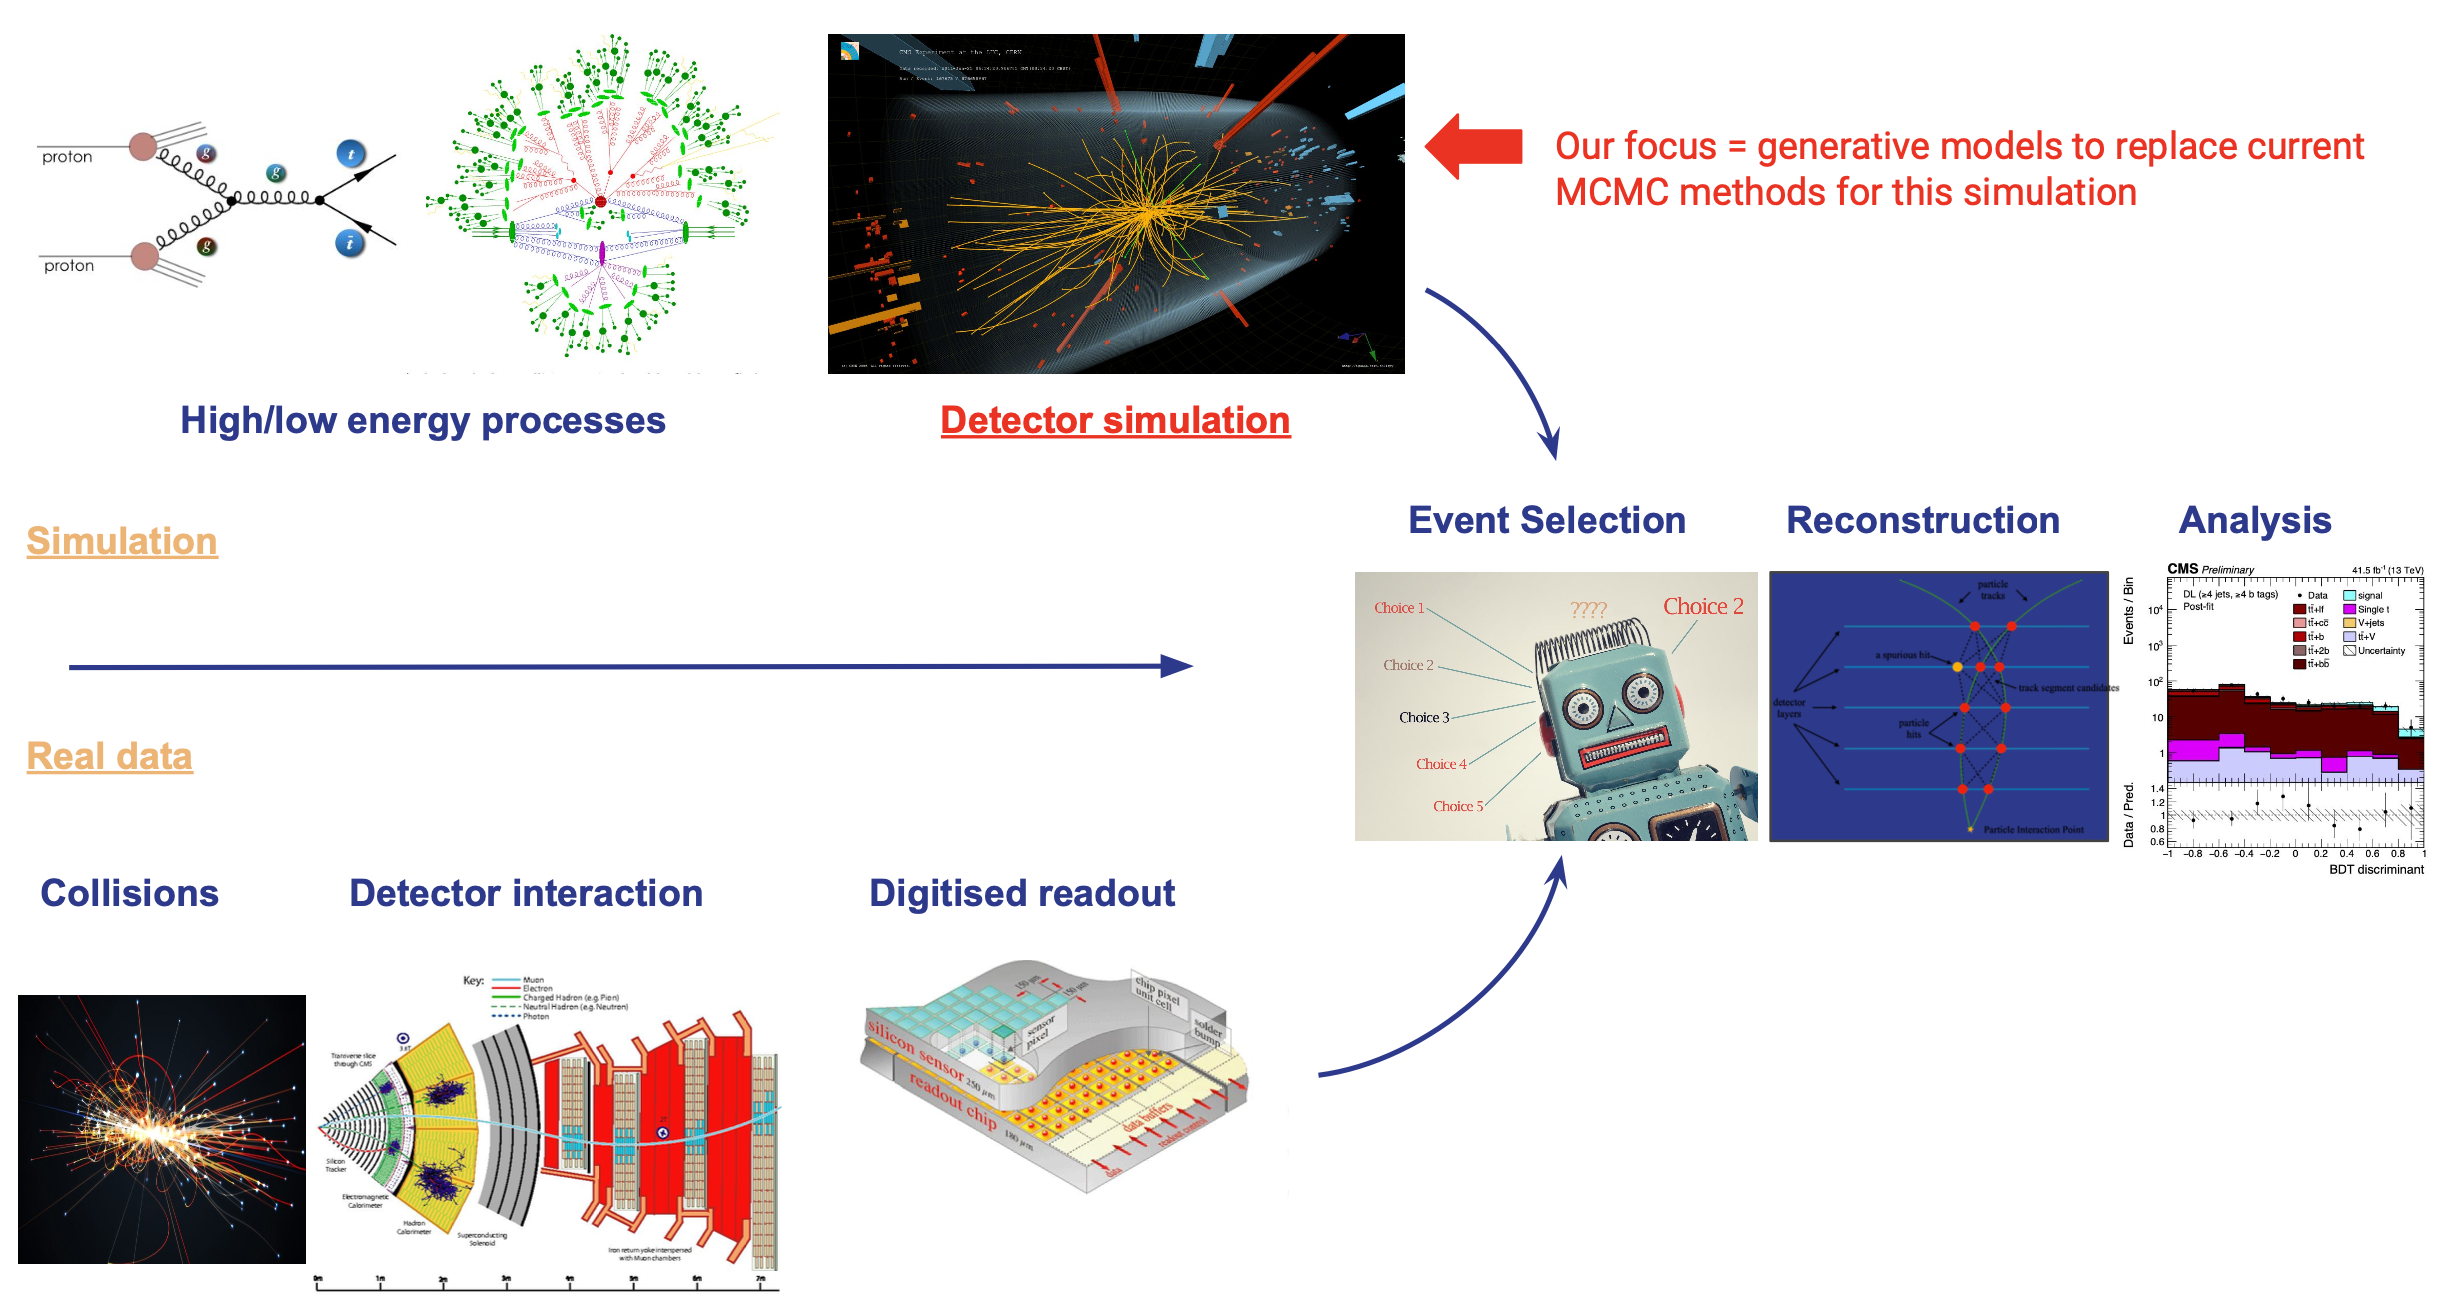
\includegraphics[width=0.7\textwidth]{Figures/simulation.png}
    \caption{The importance of simulation. Credit: Joshuha Thomas-Wilsker}
    \label{fig:fig1}
    \end{figure}

\subsection{Generative Models for Fast Simulation}
To address these challenges, generative models—particularly diffusion models—have emerged as promising alternatives for accelerating simulation while maintaining accuracy. Instead of replacing Geant4 entirely, the goal is to find an optimal balance between speed and precision, as illustrated in Figure \ref{fast}. Recent works, such as Yang et al.'s score-based models~\cite{song2020} and diffusion-based calorimeter simulations~\cite{mikuni2021}, have significantly reduced computation time while preserving fidelity. Building on these advances, our project introduces a novel model that generates 3D point clouds representing energy distributions across spatial coordinates in a single step. Unlike previous models, which often focus on one-dimensional projections (e.g., energy vs. z-coordinate), our approach captures full 3D distributions in a single forward pass, enabling rapid and comprehensive simulations suited to high-luminosity experiments.

Deep learning offers a compelling alternative to traditional parametric models, with generative techniques such as Generative Adversarial Networks (GANs)~\cite{goodfellow2014}, Variational Autoencoders (VAEs)~\cite{kingma2013}, and Normalizing Flows (NFs) ~\cite{dinh2016} increasingly adopted for fast detector simulations. GANs, for example, have demonstrated considerable success in generating calorimeter showers~\cite{paganini2018} and are now integrated into the ATLAS fast simulation framework~\cite{atlas2018}. However, they present optimization challenges and can suffer from mode collapse, where the generator fails to fully capture data diversity. NFs, while offering stable training and accurate density estimation, remain computationally expensive for high-dimensional data, limiting their feasibility for complex detector simulations. Additionally, their rigid model structure further constrains adaptability~\cite{verheyen2021, verheyen2021b}.

\subsection{Score-Based Generative Models for Simulation}
This work explores score-based generative models~\cite{song2020}, which learn the gradient of the data density rather than the density itself. This approach allows for more flexible network architectures without requiring Jacobian computation during training, enabling the use of bottleneck layers to reduce trainable parameters and improve scalability. Recent advancements in score-based models have demonstrated their potential in calorimeter simulation, achieving a balance between high-dimensional fidelity and computational efficiency—making them suitable for ultra-fine calorimeters and complex datasets~\cite{cms2017, cms2018}.

By leveraging score-based models, our project aims to address both the computational challenges of high-luminosity LHC experiments and the limitations of traditional fast simulation methods. Our approach enhances accuracy by capturing full 3D spatial distributions while significantly reducing simulation time, offering a scalable and reliable solution for next-generation collider experiments.

\begin{figure}[H]
\centering
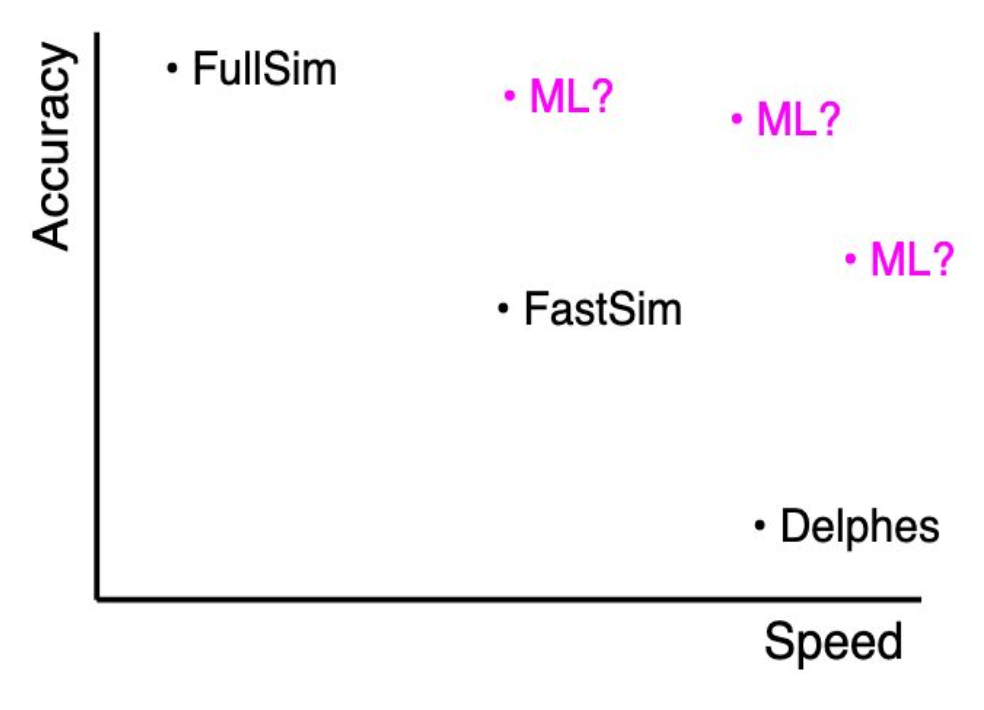
\includegraphics[width=0.7\textwidth]{Figures/fast.png}
\caption{The balance between accuracy and speed in simulation. Credit: Joshuha Thomas-Wilsker}
\label{fast}
\end{figure}

\section{Challenges}

Generating a 3D point cloud to accurately model energy deposition across spatial coordinates presents several key challenges. Traditional approaches primarily focus on one-dimensional projections, modeling energy as a function of a single spatial dimension. While effective for simplified representations, these methods fail to capture the full complexity of particle interactions. Our model, in contrast, aims to reconstruct the complete three-dimensional energy distribution in a single forward pass, requiring a delicate balance between high-dimensional fidelity and computational efficiency.

To achieve this, we integrate advanced architectural components, including Gaussian Fourier Projection for time encoding and mean-field attention mechanisms with a class token, along with conditional guidance based on incident energy. These features enable precise control over both positional and energy distributions, addressing the intricate dependencies within the 3D spatial domain. However, training a model to learn the complex correlations between spatial coordinates, energy deposition, and incident energy introduces significant computational challenges. Ensuring that the model generalizes well across various particle types and energies, while maintaining efficiency, remains a non-trivial task.

The high-dimensional nature of this generative task demands careful conditioning to reflect realistic energy variations across spatial coordinates. Our approach requires the model to dynamically adjust its predictions based on incident energy, detector response, and local correlations. This complexity leads to a tradeoff: increasing fidelity often incurs substantial computational
costs. Optimizing the architecture to maintain accuracy while reducing inference time is a key focus of our work.

Despite these challenges, our optimized approach achieves up to a 500-fold speedup over traditional Geant4-based simulations, offering a scalable alternative suited for next-generation collider experiments. By leveraging modern generative techniques, we not only enhance simulation efficiency but also improve the resolution and realism of synthetic data.

In summary, our model represents a step forward in 3D point cloud generation for high-energy physics simulations. By bridging the gap between scalability and fidelity, we address the computational limitations of conventional methods while enabling high-precision modeling of energy deposition patterns. These advancements pave the way for more efficient and realistic simulations, crucial for meeting the demands of high-luminosity experiments and future discoveries in particle physics.
